\def \currentAuthor {Gabi Sorglos} %so kann jederzeit der Autor geändert werden -> wird in der Fusszeile angezeigt.

\chapter*{Einleitende Bemerkungen}

\chapter*{Notationen}
Beschreibung wie Code, Hinweise, Zitate etc. formatiert werden  

\chapter{Einleitung}

\chapter{Projektmanagement}

\section{Metainformationen}
\subsection{Team}
\subsection{Betreuer}
\subsection{Partner}
\subsection{Ansprechpartner}
\section{Vorerhebungen}
\subsection{Projektzieleplan}
Projektziele-Hierarchie - SMART
\subsection{Projektumfeld}
\begin{itemize}
	\item Identifikation der Stakeholder
	\item Charakterisierung der Stakeholder
	\item Maßnahmen
	\item Grafische Darstellung des Umfeldes
\end{itemize}
\subsection{Risikoanalyse}
\begin{itemize}
	\item Risikomatrix
\end{itemize}
\section{Pflichtenheft}
\subsection{Zielbestimmung}
\begin{itemize}
	\item Projektbeschreibung
	\item IST-Zustand
	\item SOLL-Zustand
	\item NICHT-Ziele (Abgrenzungskriterien)
\end{itemize}
\subsection{Produkteinsatz und Umgebung}
\begin{itemize}
	\item Anwendungsgebiet
	\item Zielgruppen
	\item Betriebsbedingungen
	\item Hard-/Softwareumgebung
\end{itemize}
\subsection{Funktionalitäten}
\begin{itemize}
	\item MUSS-Anforderungen
	\begin{itemize}
		\item Funktional
		\item Nicht-funktional
	\end{itemize}
	\item KANN-Anforderungen
	\begin{itemize}
		\item Funktional
		\item Nicht-funktional
	\end{itemize}
\end{itemize}
\subsection{Testszenarien und Testfälle}
\begin{itemize}
	\item Beschreibung der Testmethodik
	\item Testfall 1
	\item Testfall 2
	\item \ldots
\end{itemize}
\subsection{Liefervereinbarung}
\begin{itemize}
	\item Lieferumfang
	\item Modus
	\item Verteilung(Deployment)
\end{itemize}
\section{Planung}
\subsection{Projektstrukturplan}
\subsection{Meilensteine}
\subsection{Gant-Chart}
\subsection{Abnahmekriterien}
\subsection{Pläne zur Evaluierung}
\subsection{Ergänzungen und zu klärende Punkte}

\chapter{Vorstellung des Produktes}
Vorstellung des fertigen Produktes anhand von Screenshots, Bildern, Erklärungen.

\chapter{Eingesetzte Technologien}
\begin{itemize}
	\item Kurzbeschreibung aller Technologien, die verwendet wurden.
	\item Technologien die aus dem Unterricht bekannt sind, nur nennen und deren  Einsatzzweck im Projekt beschreiben, nicht die Technologien selbst.
	\item Technologien die aus dem Unterricht nicht bekannt sind, im Detail beschreiben incl. deren Einsatz im Projekt
	\item Fokus aus eingesetzten Frameworks
\end{itemize}

\chapter{Problemanalyse}
\section{USE-Case-Analyse}
\begin{itemize}
	\item UseCases auf Basis von Benutzerzielen identifizieren: 
	\begin{itemize}
		\item Benutzer eines Systems identifizieren
		\item Benutzerziele identifizieren (Interviews)
		\item Use-Case-Liste pro Benutzer definieren
	\end{itemize}
	\item UseCases auf Basis von Ereignissen identifizieren: 
	\begin{itemize}
		\item Externes Event triggert einen Prozess
		\item zeitliches Event triggert einen Prozess (Zeitpunkt wird erreicht) 
		\item State-Event (Zustandsänderung im System triggert einen Prozess)
	\end{itemize}
	\item Werkzeuge:
	\begin{itemize}
		\item USE-Case-Beschreibungen (textuell, tabellarisch)
		\item USE-Case-Diagramm
		\item Aktivitätsdiagramm für den Use-Case (Interaktion zwischen Akteur und System abbilden)
		\item System-Sequenzdiagramm (Spezialfall eines Sequenzdiagramms: Nur 1 Akteur und 1 Objekt, das Objekt ist das komplette System, es geht um die Input/Output Requirements, die abzubilden sind)
	\end{itemize}
\end{itemize}

\section{Domain-Class-Modelling}
\begin{itemize}
	\item "Dinge" (Rollen, Einheiten, Geräte, Events etc.) identifizieren, um die es im Projekt geht
	\item ER-Modellierung oder Klassendiagramme
	\item Zustandsdiagramme (zur Darstellung des Lebenszyklus von Domain-Klassen darstellen)
\end{itemize}

\section{User-Interface-Design}
\begin{itemize}
	\item Mockups
	\item Wireframes
\end{itemize}


\chapter{Systementwurf}

\section{Architektur}

\subsection{Design der Komponenten}

Darstellung und Beschreibung der Systemarchitektur;

\begin{itemize}
	\item  statische Zerlegung des Systems in seine physischen Bestandteile (Komponenten, Komponentendiagramm)
	\item (textuelle) Beschreibung des dynamischen Zusammenwirkens aller Komponenten 
	\item (textuelle) Beschreibung der Strategie für die Architektur, d. h. wie die Architektur in Statik und Dynamik funktionieren soll.
	\item Verwendung von Referenzarchitekturen bzw. Architekturmustern (als Schablonen, z.B. MVC. Plugin, Pipes and Filters)
	\begin{itemize}
		\item MVC
		\item Schichten
		\item Pipes
		\item Request Broker
		\item Service-Oriented
	\end{itemize}
\end{itemize}

\subsection{Benutzerschnittstellen} 
\begin{itemize}
	\item Design des UIs
	\item Dialoge, Dialogsteuerung, Ergonomie, Gestaltung, Eingabeüberprüfungen
\end{itemize}

\subsection{Datenhaltunskonzept}
\begin{itemize}
	\item Design der Datenbank (ER-Modell)
	\item Design des Zugriffs auf diese Daten (Datenhaltungskonzept)
	\item Caching, Transaktionen
\end{itemize}

\subsection{Konzept für Ausnahmebehandlung}
\begin{itemize}
	\item Systemweite Festlegung, wie mit Exceptions umgegangen wird
	\item Exceptions sind primär aus den Bereichen UI, Persistenz, Workflow-Management
\end{itemize}

\subsection{Sicherheitskonzept}
Beschreibung aller sicherheitsrelevanten Designentscheidungen

\begin{itemize}
	\item Design der Security-Elemente
	\item Design von Safety-Elementen (Fehlertoleranz, Verfügbarkeit etc.)
\end{itemize}

\subsection{Design der Testumgebung}
\begin{itemize}
	\item wie wird getestet (Unit-Testing, Integrationstesting, Systemtests, Akzeptanztests)
	\item Testumgebung, Testprozess, Teststrategie, Testmethoden, Testfälle
\end{itemize}


\subsection{Desing der Ausführungsumgebung}
\begin{itemize}
	\item Deployment (DevOps)
	\item Betrieb (besonders Hoch- und Hertunerfahren der Anwendung)
\end{itemize}

\section{Detailentwurf}

Design jedes einzelnen USE-Cases

\begin{itemize}
	\item Design-Klassendiagramme vom Domain-Klassendiagramm ableiten (incl. detaillierter Darstellung und Verwendung von Vererbungshierarchichen, abstrakten Klassen, Interfaces)
	\item Sequenzdiagramme vom System-Sequenz-Diagramm ableiten
	\item Aktivitätsdiagramme
	\item Detaillierte Zustandsdiagramme für wichtige Klassen
\end{itemize}

Verwendung von CRC-Cards (Class, Responsibilities, Collaboration) für die Klassen
\begin{itemize}
	\item um Verantwortlichkeiten und Zusammenarbeit zwischen Klassen zu definieren und
	\item um auf den Entwurf der Geschäftslogik zu fokussieren
\end{itemize}

Design-Klassen für jeden einzelnen USE-Case können z.B. sein:

\begin{itemize}
	\item UI-Klassen
	\item Data-Access-Klassen
	\item Entity-Klassen (Domain-Klassen)
	\item Controller-Klassen
	\item Business-Logik-Klassen
	\item View-Klassen
\end{itemize}

Optimierung des Entwurfs (Modularisierung, Erweiterbarkeit, Lesbarkeit):

\begin{itemize}
	\item Kopplung optimieren
	\item Kohäsion optimieren
	\item SOLID
	\item Entwurfsmuster einsetzen
\end{itemize}

\chapter{Implementierung}
Detaillierte Beschreibung der Implementierung aller Teilkomponenten der Software entlang der zentralsten Use-Cases:
\begin{itemize}
	\item GUI-Implementierung
	\item Controllerlogik
	\item Geschäftslogik
	\item Datenbankzugriffe
\end{itemize}


Detaillierte Beschreibung der Teststrategie (Testdriven Development):

\begin{itemize}
	\item UNIT-Tests (Funktional)
	\item Integrationstests
\end{itemize}

Zu Codesequenzen:
\begin{itemize}
	\item kurze Codesequenzen direkt im Text (mit Zeilnnummern auf die man in der Beschreibung verweisen kann)
	\item lange Codesequenzen in den Anhang (mit Zeilennummer) und darauf verweisen (wie z.B. hier \cref{qj})
\end{itemize}

\def \currentAuthor {Florian Tipotsch}

\section{Webapp}

Für unser Projekt erstellen wir eine Webapp mit der man die Daten seiner eigenen Zuchtkammer anzeigen lassen kann.
Wir haben geplant das man sich mit der Seriennummer der Box Registrieren kann und dann am Handy über eine Webapp alle Daten anzeigen lassen kann. Folgende Daten sollte man auslesen können:

\begin{itemize}
	\item Sauerstoff
	\item Luftfeuchtigkeit
	\item Gewicht
	\item Futtermenge
	\item ungefähre Zeit bis zu Reife
\end{itemize}

\newpage
\def \currentAuthor {Kevin Glatz}
\newpage


\section{Verkablung}

Die Verkablung der einzelnen Module ist aus verschiedenen Gründen wichtig. Zum einen brauch jedes Modul genügend Strom um seine Aufgabe zu erfüllen, gleichzeitig würde es aber ohne die Erdung zu einem Kurzschluss kommen. Des weiteren ist es wichtig das die Module Daten auslesen und weitersenden können

\subsection{Aufbau}

(bild einfügen)

In Abbildung x können wir nun den Arduino und das Breadboard sehen.  Dort kann man direkt die drei Farben erkennen die jeweils für Stromzufuhr (blau), Datenauslesung (grün) und Erdung (braun) stehen.

(bild mit stromfluss einfügen)

Hier sieht man wie der Strom im Breadboard fließt. Das heißt wenn man in der Untersten Reihe das Board mit 5 Volt versorgt sind alle weiteren Steckplätze verwendbar. Wichtig hierbei ist, dass das Kabel für die Stromzufuhr auch auf der richtigen Reihe platziert wurde. Das erkennt man bei dieser Leiterplatte an dem Plus und Minus Zeichen Plus steht hierbei für Strom und Minus für die Erdung.

Falls man das Falsch verkabelt funktioniert das Modul nicht, es werden allerdings keine Schäden angerichtet


(Bild mit analog und digitalwerten einfügen)

Der Arduino hat zwei Möglichkeiten Daten auszulesen. Einmal spricht man hier von digitaler und analogen Datenauslesung. (internet suche) Digitale Werte bedeutet hier allerdings nur das der ausgelesene Wert als 0 oder 1 abgespeichert werden kann, analoge Daten sind bei diesem Punkt anders, da diese einen Wert zwischen 0 und x haben können (zitat)

\section{Programmierung}

Um die Daten der einzelnen Sensoren verwenden zu können, müssen diese ausgelesen und sinnvoll wiedergegeben werden. Nur sobald die Sensoren richtig Programmiert und verkabelt sind, kriegt man lesbare Information. Diese können anschließend weiter interpretiert und verwendet werden. 

Die verwendeten Sensoren:

\begin{itemize}
	\item DHT11
	\item CCS811
	\item Hebel
	\item Servo SG90
	\item photocell
\end{itemize}


\subsection{DHT11 \& CCS811}

Für den DHT 11 sowie dem CCS811 gibt es eine von Adafruit frei verwendbare Bibliothek. Mithilfe von dieser kann man ein Objekt erstellen und es mithilfe diesem Objektes die Momentane Temperatur/Luftfeuchtigkeit auslesen.


	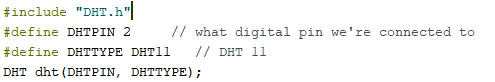
\includegraphics[width=1\linewidth]{../Bilder/Programmierung/define(DHTCCS)}



Das \#include fügt die Klasse in unser Projekt ein und erlaubt es uns das Objekt dht sowie ccs zu erstellen.

Das \#define legt des weiteren fest, dass relevante Daten, im Falle des DHT Moduls, von Pin 2 kommen. 


	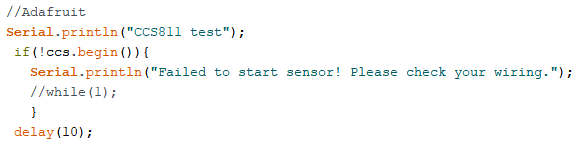
\includegraphics[width=1.2\linewidth]{../Bilder/Programmierung/setup(CCS)}



Die Setup Funktion, wird für einmalige Dinge wie die Kalibrierung, dem Starten des Serial Monitors oder der Verbindung mit dem Raspberry verwendet. Der CO2 Sensor benötigt das Setup, da es zuerst kalibriert werden muss um die Luftqualität zu messen.

	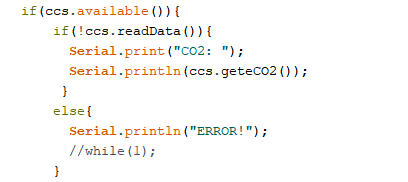
\includegraphics[width=0.9\linewidth]{../Bilder/Programmierung/loop(DHTCCS)}



Die Loop Funktion, wiederholt sich im vorgegebenen Rhythmus immer wieder und gibt keine Variablen zurück. Dort können werden alle Daten ausgelesen und an das WLAN Modul weitergeschickt bzw. in diesem Fall wird es auf den Serial Monitor ausgegeben.

Die WENN abfrage prüft als erstes ob der CO2 Sensor kalibriert wurde oder nicht. Falls es gelungen sein sollte gibt es die Werte mit dem Befehl Serial.println(ccs.geteCO2()); im Serial Monitor aus.

\subsection{Hebel}

Das Joystick bzw. der Hebel konnte direkt abgelesen werden. Wichtig hierbei ist es das man nicht nur eine Achse im Setup verwendet sondern beide, ansonsten kommt es bei dem Loop zu einem Fehler und der Wert der benötigten Achse verändert sich nicht.


\subsection{SG90}

Die vom verwendeten Bibliotheken waren bei der Installierung der Arudino eigenen IDE direkt dabei. Die Servo kontrolliert die Luftzuvor und muss daher Werte vom CCS811 wiederverwenden

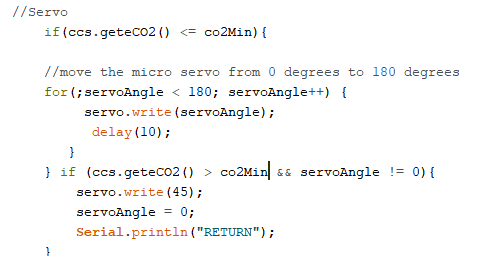
\includegraphics[width=1\linewidth]{../Bilder/Programmierung/loop(SG)}

Die If Abfrage prüft ob CO2 einen Mindestwert (co2Min) unterschreitet. Falls das passiert  wird eine Schleife ausgeführt die den Servo 180° dreht. Diese 180° würde die Lüftungsklappe aufhalten. Falls der CO2 Wert wieder in einem akzeptablen Bereich liegt und die Position des Motors nicht null beträgt, wird die zweite Schleife aktiviert die den Motor zur Position 0 zurückbringt 


\subsection{photocell}



\def \currentAuthor {Leonid Hammer}


\chapter{Deployment}
\begin{itemize}
	\item Umsetzung der Ausführungsumgebung
	\item Deployment
	\item DevOps-Thema
\end{itemize}

\chapter{Tests}

\section{Systemtests} 
Systemtests aller implementierten Funktionalitäten lt. Pflichtenheft
\begin{itemize}
	\item Beschreibung der Teststrategie
	\item Testfall 1
	\item Testfall 2
	\item Tesfall 3
	\item …
\end{itemize}

\section{Akzeptanztests}

\chapter{Projektevaluation}
siehe Projektmanagement-Unterricht

\chapter{Benutzerhandbuch} 
falls im Projekt gefordert

\chapter{Betriebswirtschaftlicher Kontext}
BW-Teil

\chapter{Zusammenfassung}
\begin{itemize}
	\item Etwas längere Form des Abstracts
	\item Detaillierte Beschreibung des Outputs der Arbeit
\end{itemize}